\section{Methods}
\label{sec:Methods}

The call graph was provided as a labeled edge list, and was modeled as a weighted, undirected, multigraph, as shown in Fig. \ref{fig:SmallGraph}.
The graph was organized as each of the nodes being the unique identifier to a customer, with edges between the customers representing:
\begin{itemize}
	\item \texttt{days} - the number of distinct days that the two nodes communicated during the month,
	\item \texttt{calls} - the number of distinct calls that the the nodes made during the month,
	\item \texttt{secs} - the cumulative sum of all calls that the modes made during the month and,
	\item \texttt{texts} - the number of distinct texts that the two nodes made during the month.
\end{itemize}
\begin{figure}[ht]
\centering
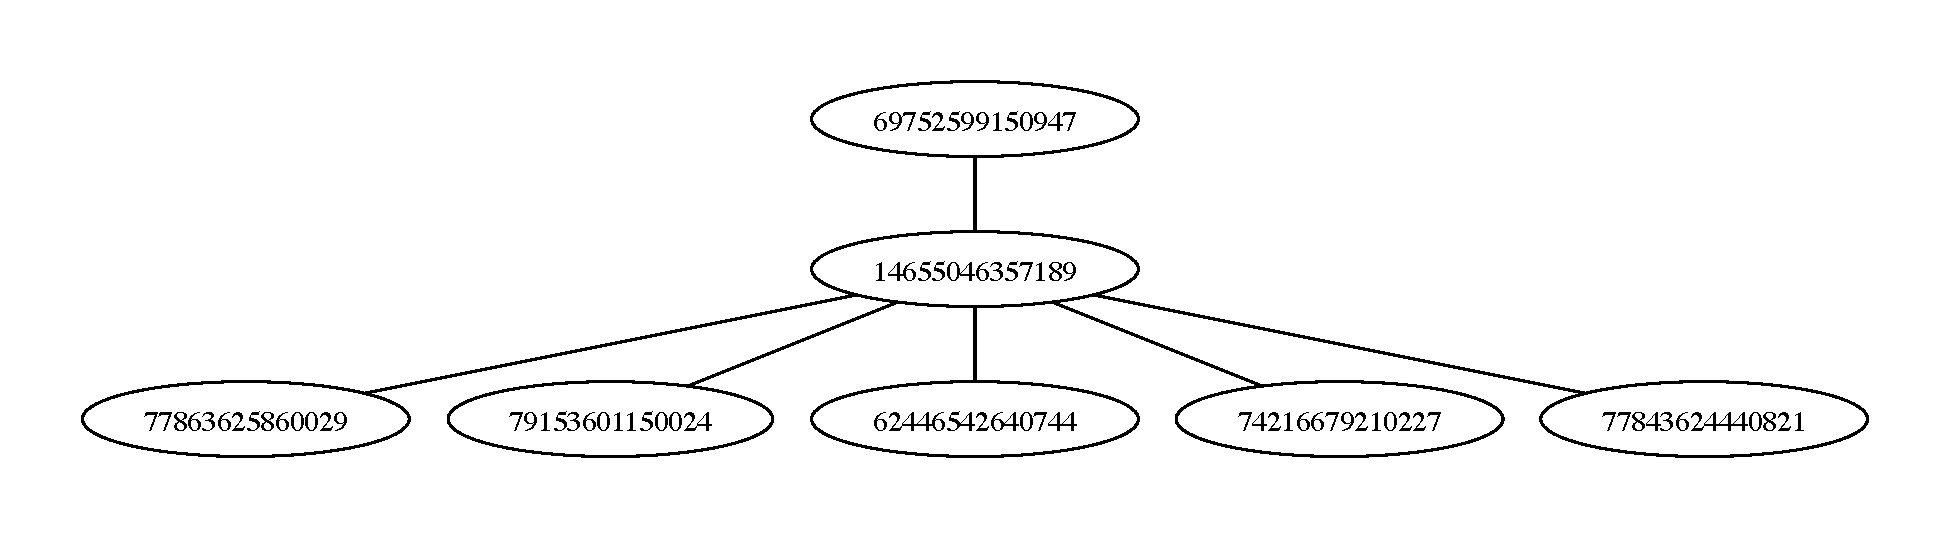
\includegraphics[width=0.45\textwidth]{SmallGraph.pdf}
\caption{Example Call Graph}
\label{fig:SmallGraph}
\end{figure} 
The data was analyzed in order to determine the distribution of calls, texts, days, and seconds for each city in order to determine the size of the problem.
It was immediately noticed that several of the callers where large outliers, these are probably robot callers in the network.
\begin{figure*}[ht!]
	\centering
	\begin{subfigure}[b]{0.45\textwidth}
		\centering
		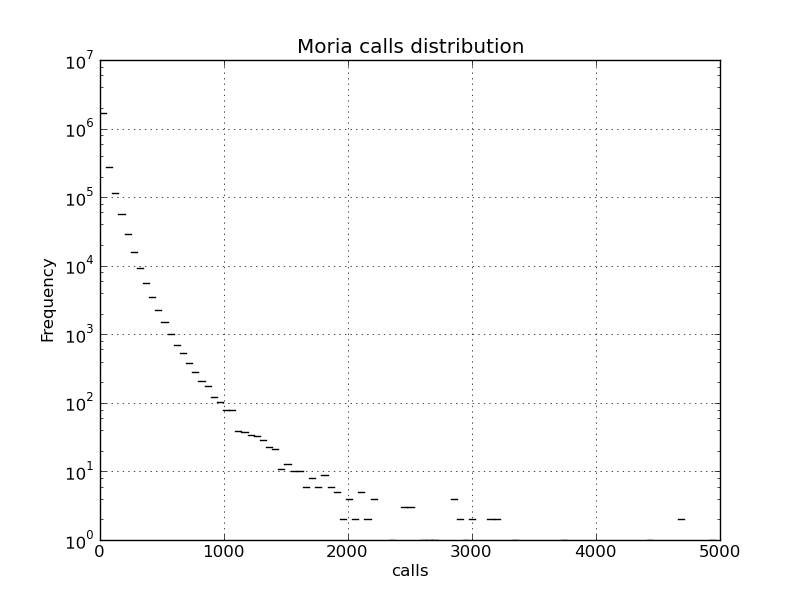
\includegraphics[width=\textwidth]{Moria_calls_distribution}
	\end{subfigure}%
	~
	\begin{subfigure}[b]{0.45\textwidth}
		\centering
		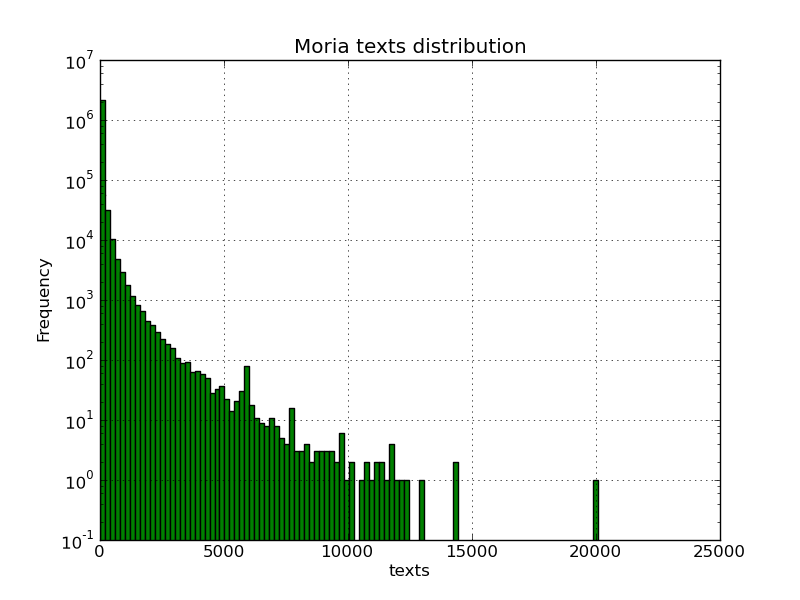
\includegraphics[width=\textwidth]{Moria_texts_distribution}
	\end{subfigure}
	

	\begin{subfigure}[b]{0.45\textwidth}
		\centering
		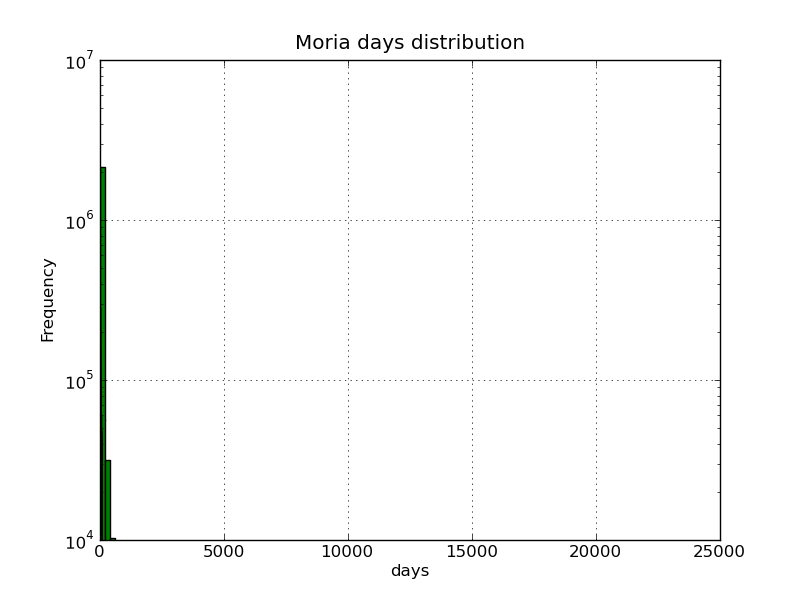
\includegraphics[width=\textwidth]{Moria_days_distribution}
	\end{subfigure}%
	~
	\begin{subfigure}[b]{0.45\textwidth}
		\centering
		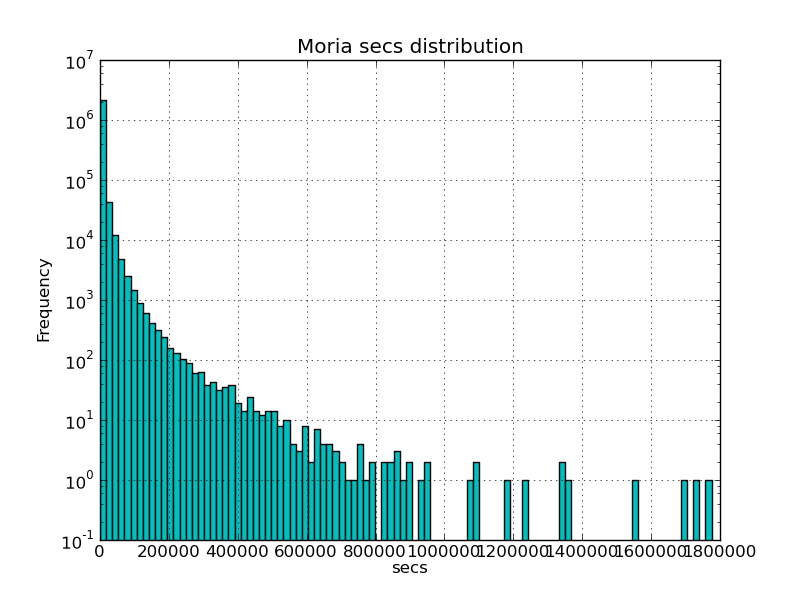
\includegraphics[width=\textwidth]{Moria_secs_distribution}
	\end{subfigure}
	\caption{Distribution of Moria Edges}
	\label{fig:MoriaEdgeDist}
\end{figure*}
\begin{figure*}[ht!]
	\centering
	\begin{subfigure}[b]{0.45\textwidth}
		\centering
		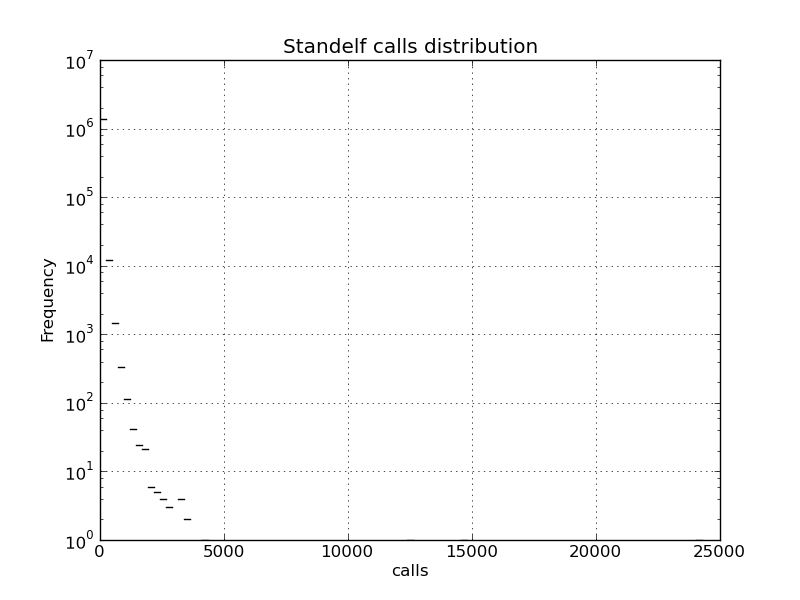
\includegraphics[width=\textwidth]{Standelf_calls_distribution}
	\end{subfigure}%
	~
	\begin{subfigure}[b]{0.45\textwidth}
		\centering
		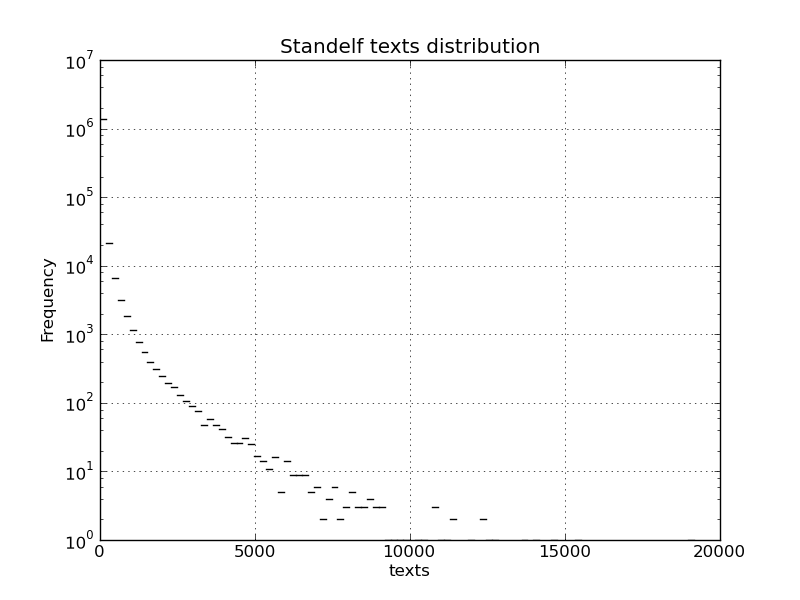
\includegraphics[width=\textwidth]{Standelf_texts_distribution}
	\end{subfigure}
	

	\begin{subfigure}[b]{0.45\textwidth}
		\centering
		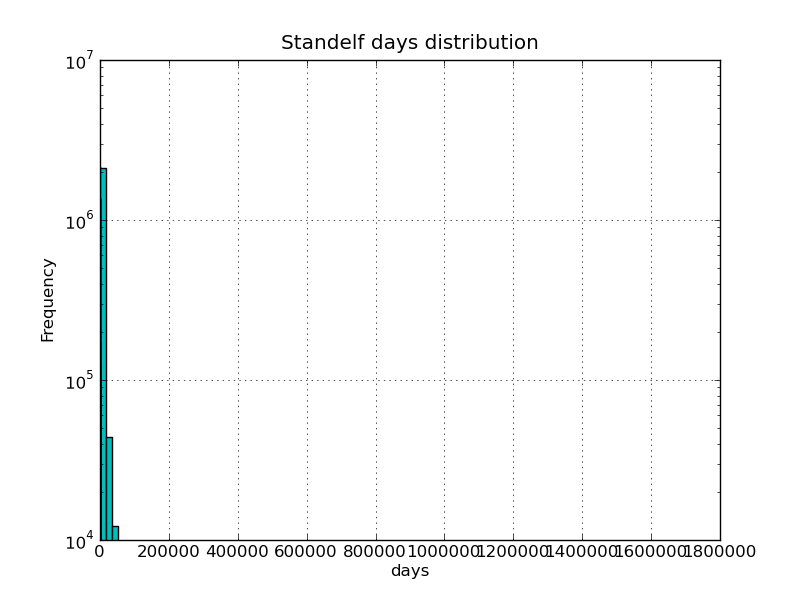
\includegraphics[width=\textwidth]{Standelf_days_distribution}
	\end{subfigure}%
	~
	\begin{subfigure}[b]{0.45\textwidth}
		\centering
		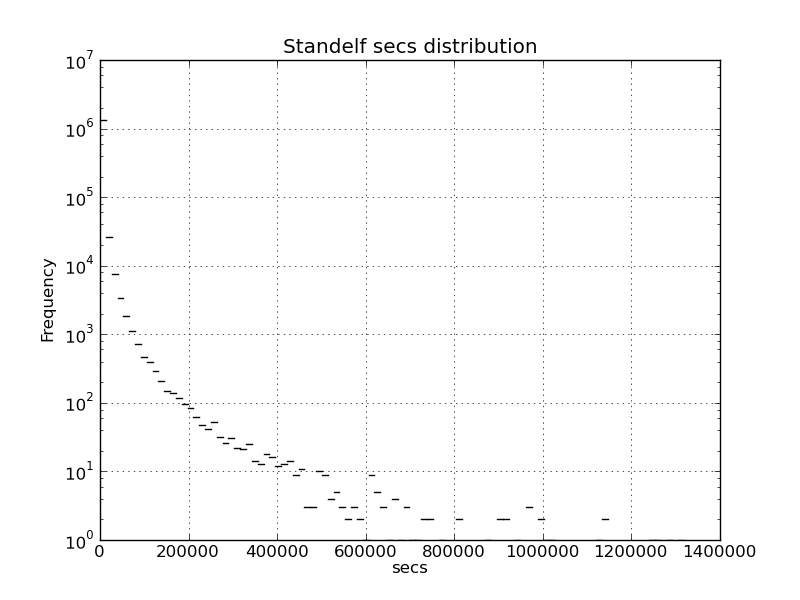
\includegraphics[width=\textwidth]{Standelf_secs_distribution}
	\end{subfigure}
	\caption{Distribution of Standelf Edges}
	\label{fig:StandelfEdgeDist}
\end{figure*}
In addition, the sum of the proprieties of the nodes were calculated by summing all of the edges into the nodes.
It is then possible to see the distribution of how people communicated for the two cities.
The degree is defined as the number of neighbors a given node has.
\begin{figure*}[ht!]
	\centering
	\begin{subfigure}[b]{0.45\textwidth}
		\centering
		\includegraphics[width=\textwidth]{Moria_calls_cum_distribution}
	\end{subfigure}%
	~
	\begin{subfigure}[b]{0.45\textwidth}
		\centering
		\includegraphics[width=\textwidth]{Moria_texts_cum_distribution}
	\end{subfigure}
	

	\begin{subfigure}[b]{0.45\textwidth}
		\centering
		\includegraphics[width=\textwidth]{Moria_degree_cum_distribution}
	\end{subfigure}%
	~
	\begin{subfigure}[b]{0.45\textwidth}
		\centering
		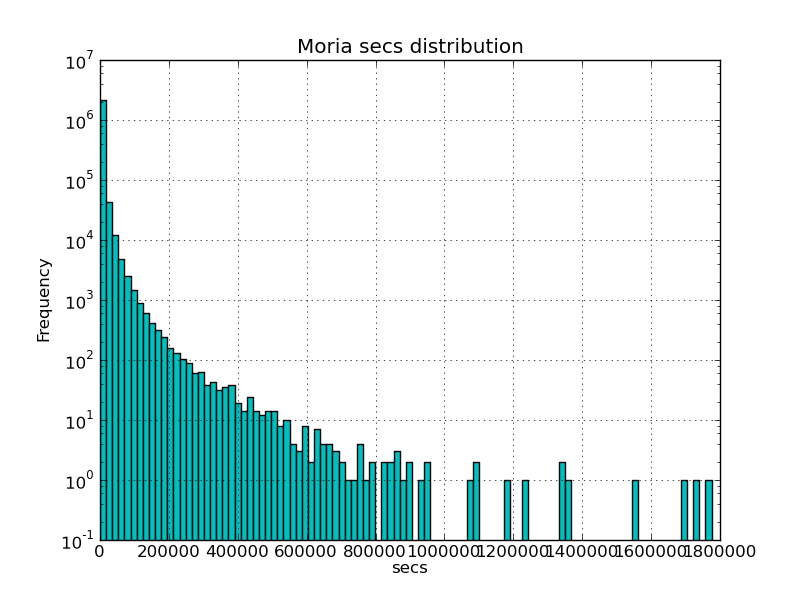
\includegraphics[width=\textwidth]{Moria_secs_distribution}
	\end{subfigure}
	\caption{Distribution of Moria Nodes}
	\label{fig:MoriaNodeDist}
\end{figure*}
\begin{figure*}[ht!]
	\centering
	\begin{subfigure}[b]{0.45\textwidth}
		\centering
		\includegraphics[width=\textwidth]{Standelf_calls_cum_distribution}
	\end{subfigure}%
	~
	\begin{subfigure}[b]{0.45\textwidth}
		\centering
		\includegraphics[width=\textwidth]{Standelf_texts_cum_distribution}
	\end{subfigure}
	

	\begin{subfigure}[b]{0.45\textwidth}
		\centering
		\includegraphics[width=\textwidth]{Standelf_degree_cum_distribution}
	\end{subfigure}%
	~
	\begin{subfigure}[b]{0.45\textwidth}
		\centering
		\includegraphics[width=\textwidth]{Standelf_secs_cum_distribution}
	\end{subfigure}
	\caption{Distribution of Moria Nodes}
	\label{fig:StandelfNodeDist}
\end{figure*}
\subsection{LSA Based Similarity Measure}
% Copied from John's email
Previous work conducted by J Martin suggested that personality profiles can be modeled with an LSA based system.
Based on this premise, it was suggested that a node (person) could be effectively "described" by the set of other people
they were connected to.  This description could then be measured for
similarity to other node descriptions and hopefully we would find that
"similar" nodes were connected. In the past work we did there was some promise
in the initial results for group analysis, but it was not pursued very far and
there were other data items that were being considered as well (and it had
nothing to do with telephone usage patterns).

This hypothesis was tested by initially constructed a sparse matrix for each of the
graph files for both the Moria and Standelf.  For each connected node, the
connection weight was determined by taking each of the 4 attribute values,
dividing by their respective standard deviation, and summing the results into
a single weight for each connection. This experiment was also completed by using a
simpler weighting scheme giving a 1 if any call was made and another 1 if any
text was made.

This sparse matrix in any case was extremely sparse, being around 0.00051\%
nonzero for Moria and 0.00059\% for Standelf.  We usually deal with matrices
that have a nonzero rate of 0.001\% to 0.01\% for text mining applications.  I
computed a truncated SVD for these sparse matrices, forming an LSA space at
approximately 250 dimensions for each.  Then using these 250 dimension spaces
I looked at comparing the first 1,000 nodes of each graph to all the other
nodes in the graph computing their vector cosine similarity and noting if the
nodes were connected or not.  This takes a while to run so there has not been
much opportunity to tweak any of the parameters, therefore it cannot be conclude
with any certainty, but the initial results do not look promising.  The first
sets that did not show any clear indication of connectivity
determined by the similarity measure.

\subsection{Artificial Neural Network Classification}
The next approach implemented was an artificial neural network classification system.
Using the \verb+PyBrain+ tool module a feed forward neural network was constructed with 8 inputs representing the edge between node \texttt{u} and \texttt{v}:
\begin{itemize}
	\item the degree of node \texttt{u},
	\item the closeness of node \texttt{u},
	\item \texttt{days} of the edge,
	\item \texttt{calls} of the edge,
	\item \texttt{secs} of the edge,
	\item \texttt{texts} of the edge,
	\item the closeness of node \texttt{v}, and,
	\item the degree of node \texttt{u}.
\end{itemize}
The closeness of node was calculated using the \verb+networkx+ module with \verb+closeness_centrality+, defined to be 1 over the average distance to all other nodes. The distances where not weighted, and all distances where normalized by the graph size.
The degree was calculated with \verb+degree+ as the the sum of the edge weights of adjacent nodes for a particular node (completed for all nodes).
The other elements of the training vector were simply filled with the values from the edge.

Training data for the neural network was then the set of all example nodes and edges presented in the target class of 1 (the edge exists). This was ultimately a flaw in the design of the neural network (or any classification based system) as discussed in Section \ref{sec:Results}.

\subsection{Spectral Approach for Finding Possible Communities in Graph}
For this call graph data set, an interesting question comes to our mind which is how to find the community structure in the graph. The cell phone users in the same community will have stronger relationship between each other than that between uses from different communities. Therefore, if we can find such communities in the call graph, it might be very helpful for us to understand the cell phone users' behavior.

The approach we use to find community structure in call graph is named spectral graph. The basic idea of this approach is to use the eigenvectors of the Laplacian matrix of the graph to partition the vertices into different clusters. Now we are going to introduce the definition of the Laplacian matrix of a graph. 

In graph $G$, let $d_v$ denote the degree of vertex $v$, the \text{Laplacian} of $G$ is defined as the matrix 
\begin{equation}
L(u,v) = \begin{cases} 1 & \text{if  $u=v$ and $d_v \ne 0$,} \\ -\frac{1}{\sqrt{d_ud_v}} & \text{if $u$ and $v$ are adjacent,} \\ 0 & \text{otherwise.}\end{cases}
\end{equation}    
Let $T$ denote the diagonal matrix with the $(v,v)$-th entry having value $d_v$. The \text{Laplacian} of $G$ can be written as 
\begin{equation}
L=I-T^{-1/2}AT^{1/2}
\end{equation}
where $A$ is the adjacency matrix of $G$ (i.e., $A(x,y)=1$ if $x$ is adjacency to $y$, and $0$ otherwise) and $I$ is an identity matrix. All matrices here are $n \times n$ where $n$ is the number of vertices in $G$.

Now let's show how to use spectral graph approach to find possible communities in graph. For example, we first import the raw data of call graph of Moria city in month 1 and generate the adjacency matrix of this call graph as shown in Fig. \ref{Moria_1_adj}.

\begin{figure}[ht]
\centering
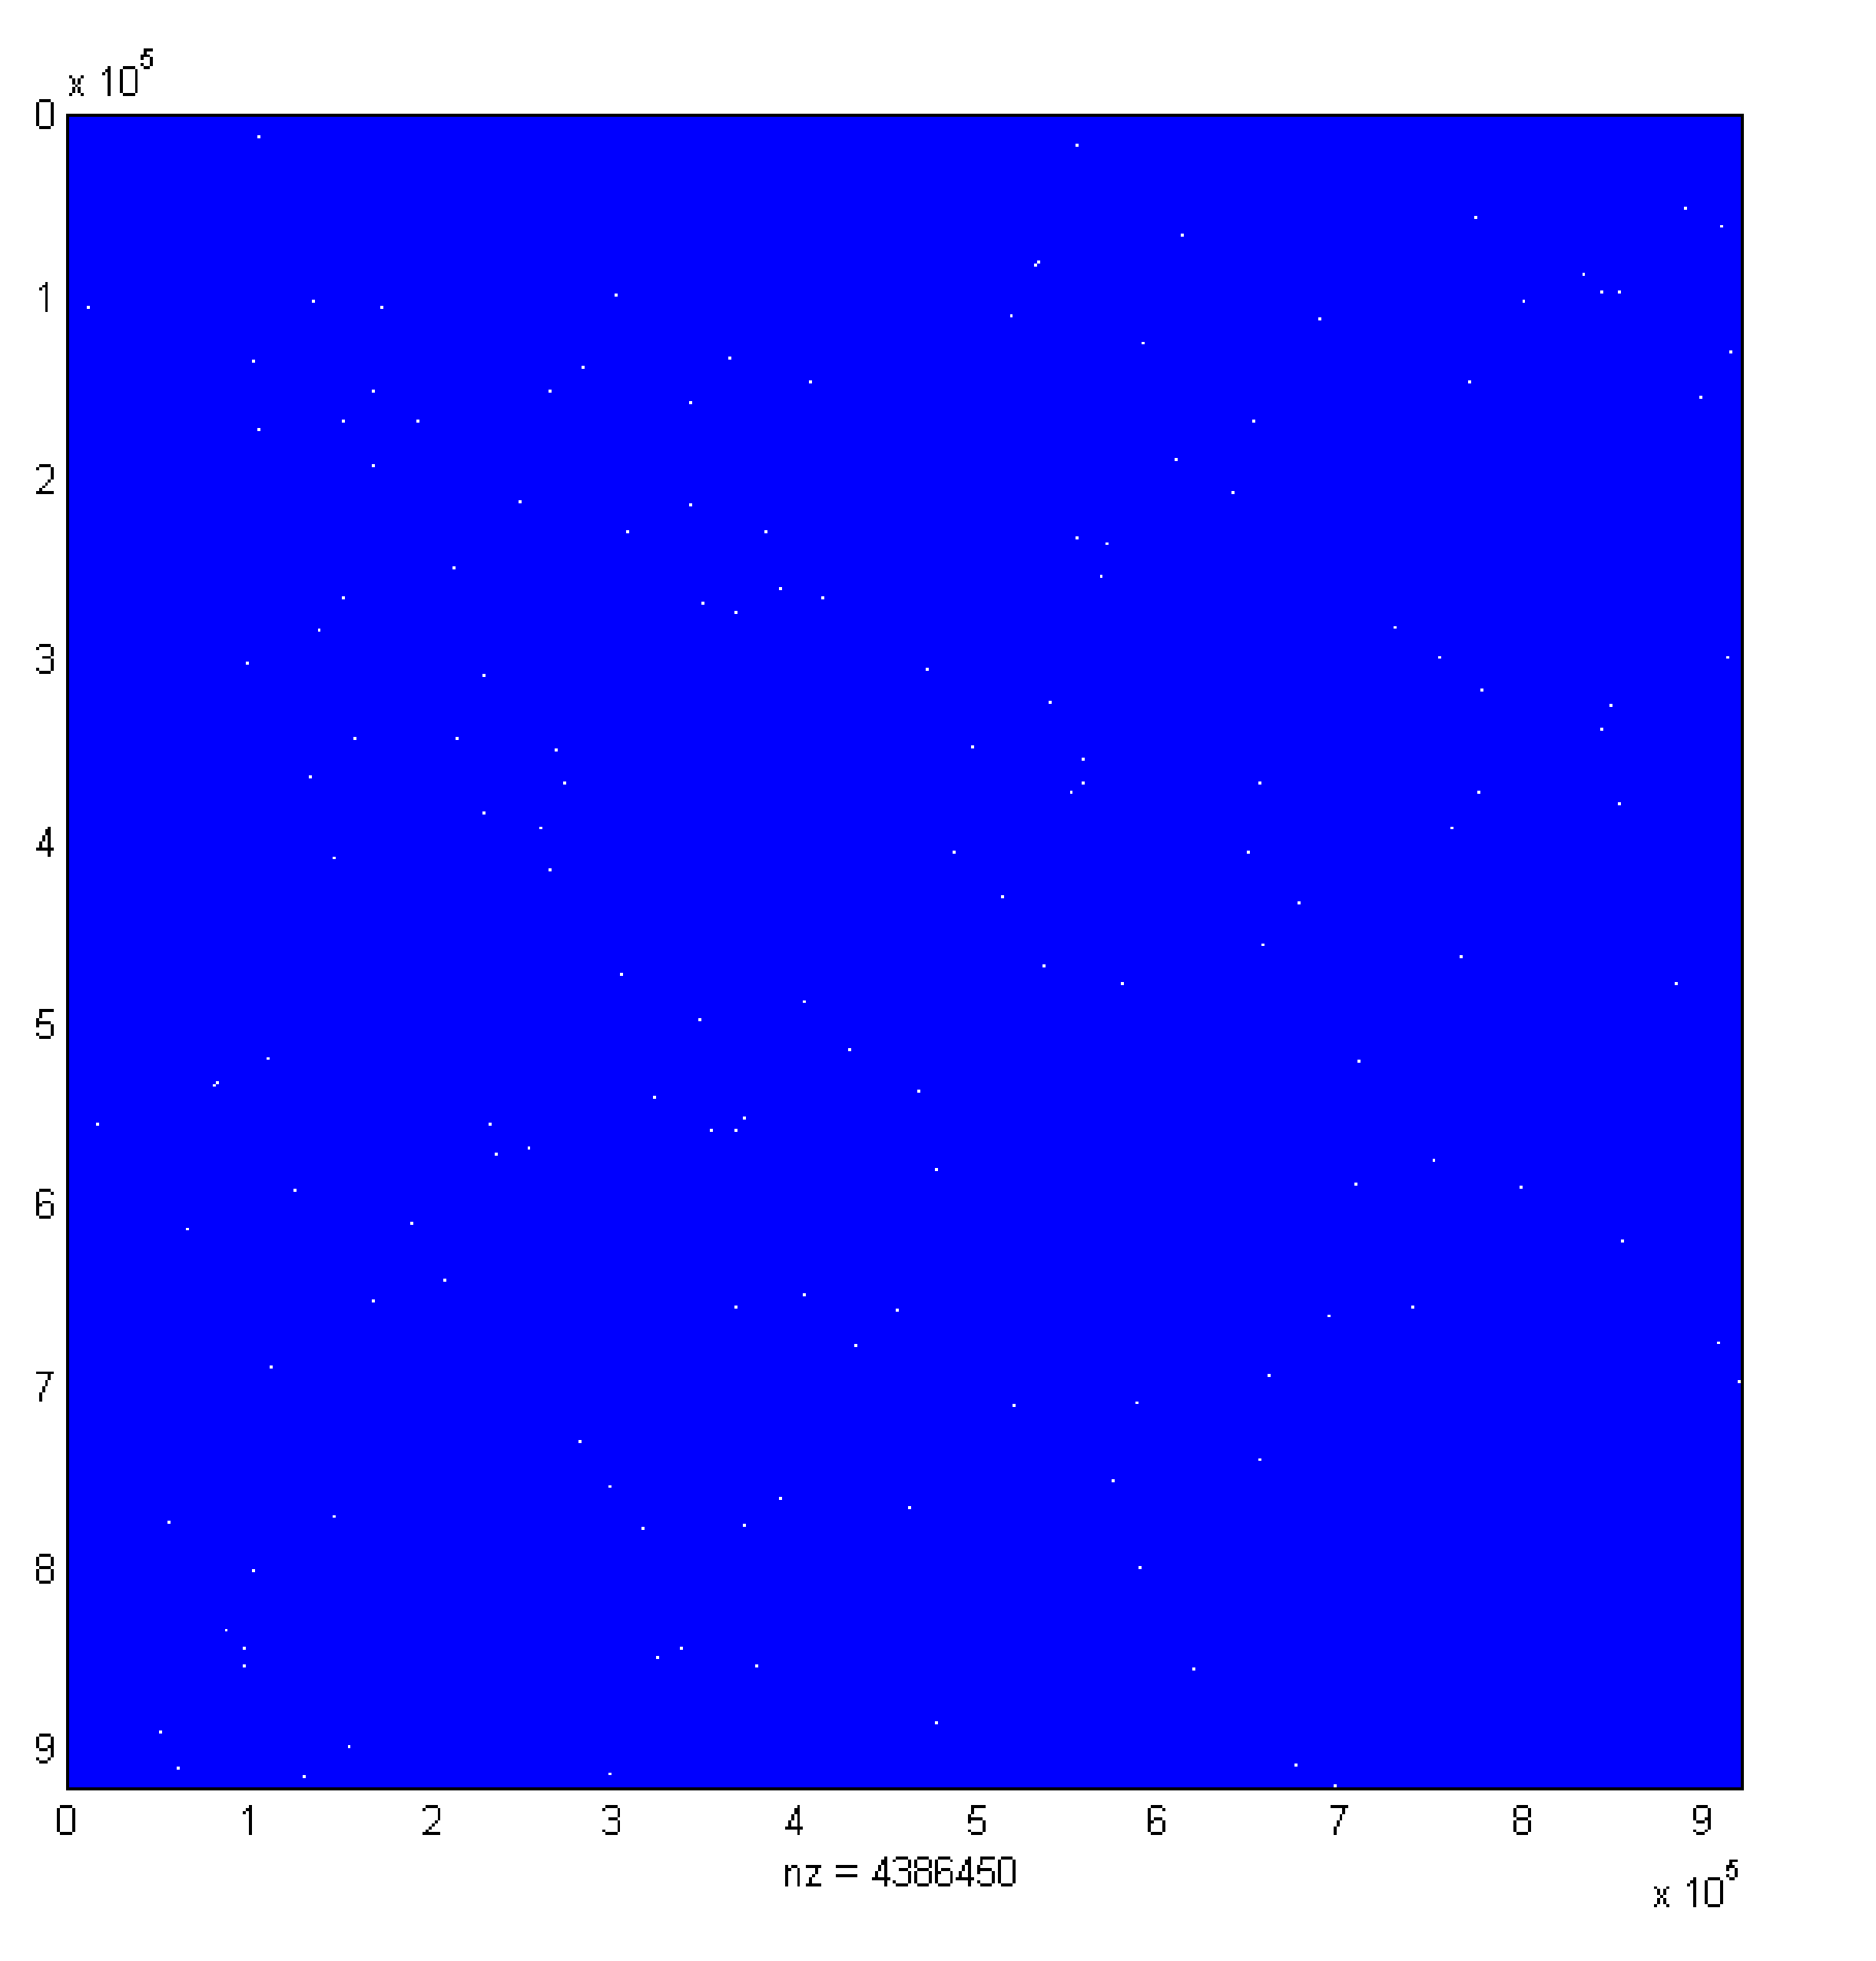
\includegraphics[width=0.45\textwidth]{Moria_1_adj.pdf}
\caption{Adjacency Matrix of Call Graph of Moria City in Month 1}
\label{Moria_1_adj}
\end{figure}  

From Fig. \ref{Moria_1_adj}, we can observe that this call graph is very dense and it is impossible for us to find any community structures in this figure because the vertices of this call graph are randomly arranged in the adjacency matrix. 

Now let's investigate what the second smallest eigenvector of the \text{Laplacian} matrix tells us about this graph. The following MATLAB code is used to compute the eigenvalues and eigenvectors of the \text{Laplacian} matrix of call graph of Moria city in month 1.

\begin{lstlisting}
Moria_1_I = speye(size(Moria_1_adj,1));
Moria_1_T = diag(sum(Moria_1_adj,2).^(-0.5));
Moria_1_L = Moria_1_I-Moria_1_T*Moria_1_adj*Moria_1_T;
[Moria_1_V,Moria_1_D] = eigs(Moria_1_L);
\end{lstlisting}

Then we sort the second smallest eigenvector and permute the vertices of this call graph based on the order of components in the sorted second smallest eigenvector.  

\begin{lstlisting}
[ignore Moria_1_p] = sort(Moria_1_V(:,2));
spy(Moria_1_adj(Moria_1_p,Moria_1_p));
\end{lstlisting} 

In the end, the \textbf{spy()} function will plot the rearranged adjacency matrix of the call graph, which is shown in Fig. \ref{Moria_1_clustered}. 

\begin{figure}[ht]
\centering
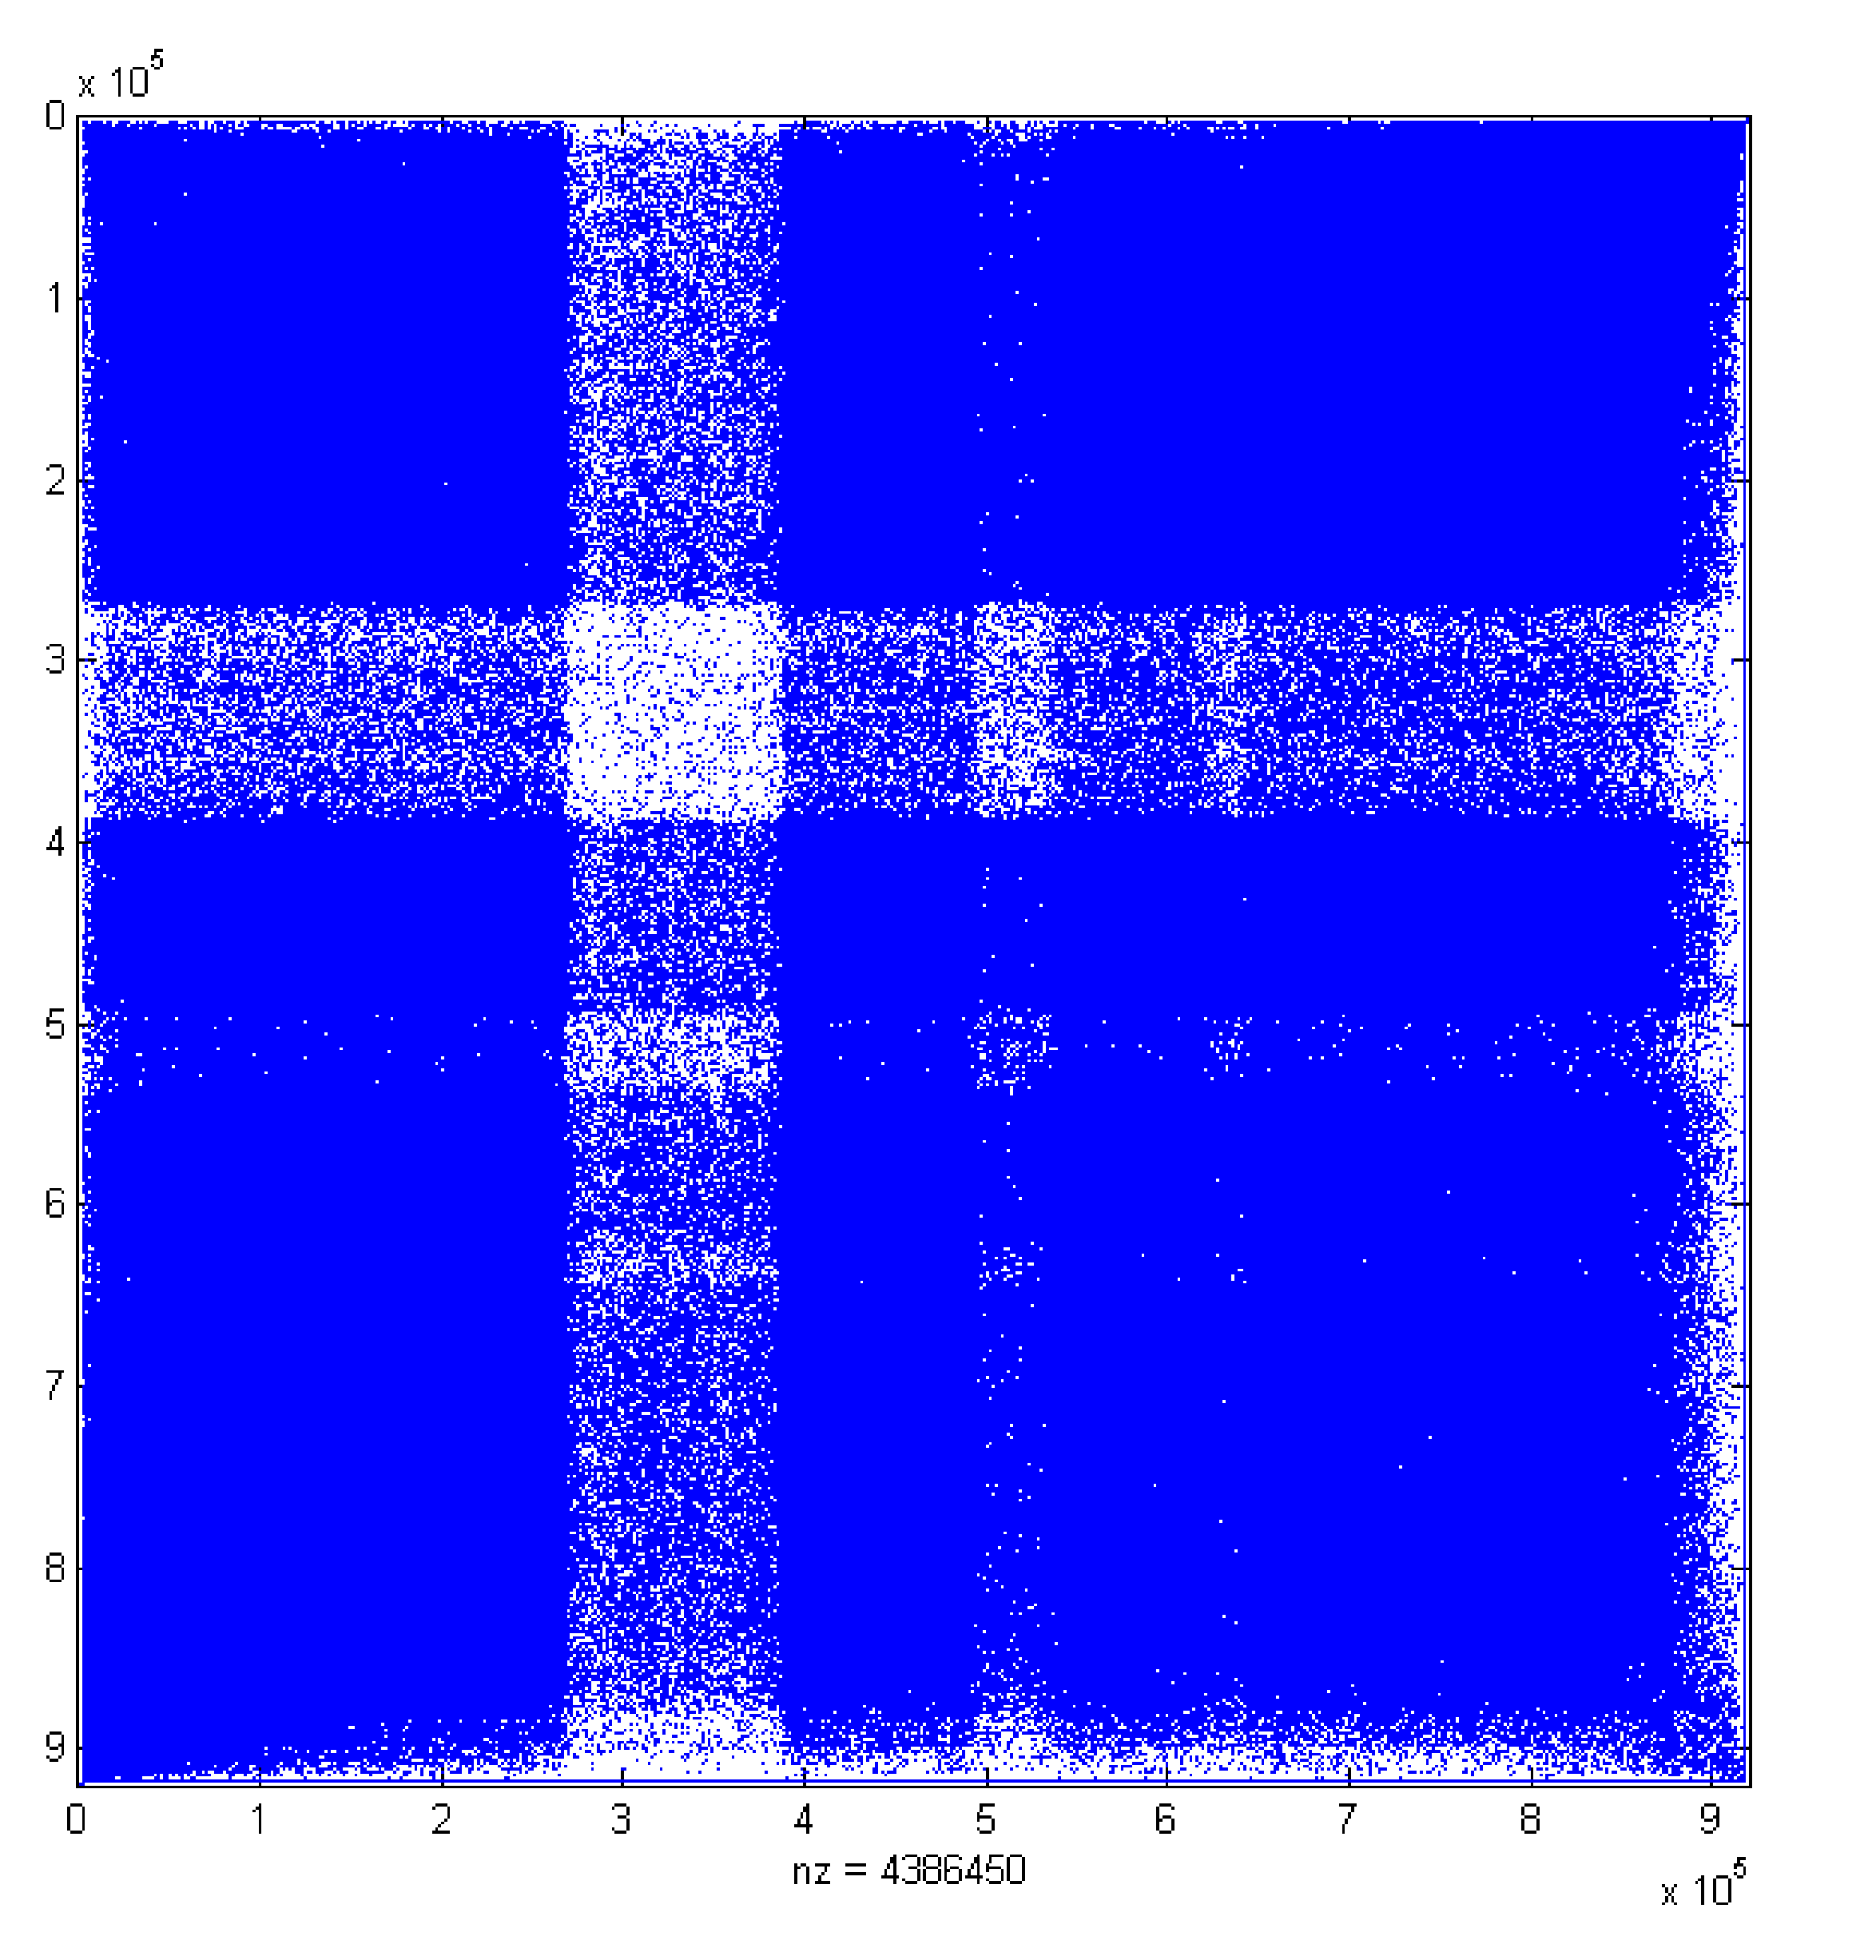
\includegraphics[width=0.45\textwidth]{Moria_1_clustered.pdf}
% where an .eps filename suffix will be assumed under latex,
% and a .pdf suffix will be assumed for pdflatex; or what has been declared
% via \DeclareGraphicsExtensions.
\caption{Rearranged Adjacency Matrix of Call Graph of Moria City in Month 1}
\label{Moria_1_clustered}
\end{figure} 

In Fig. \ref{Moria_1_clustered}, we can observe some community structure, for example, the vertices at the upper left corner of the matrix have stronger connection between each other. Similarly, we can also generate the rearranged adjacency matrix of call graph of Moria city in month 2, as shown in Figure \ref{Moria_2_clustered} 

\begin{figure}[ht]
\centering
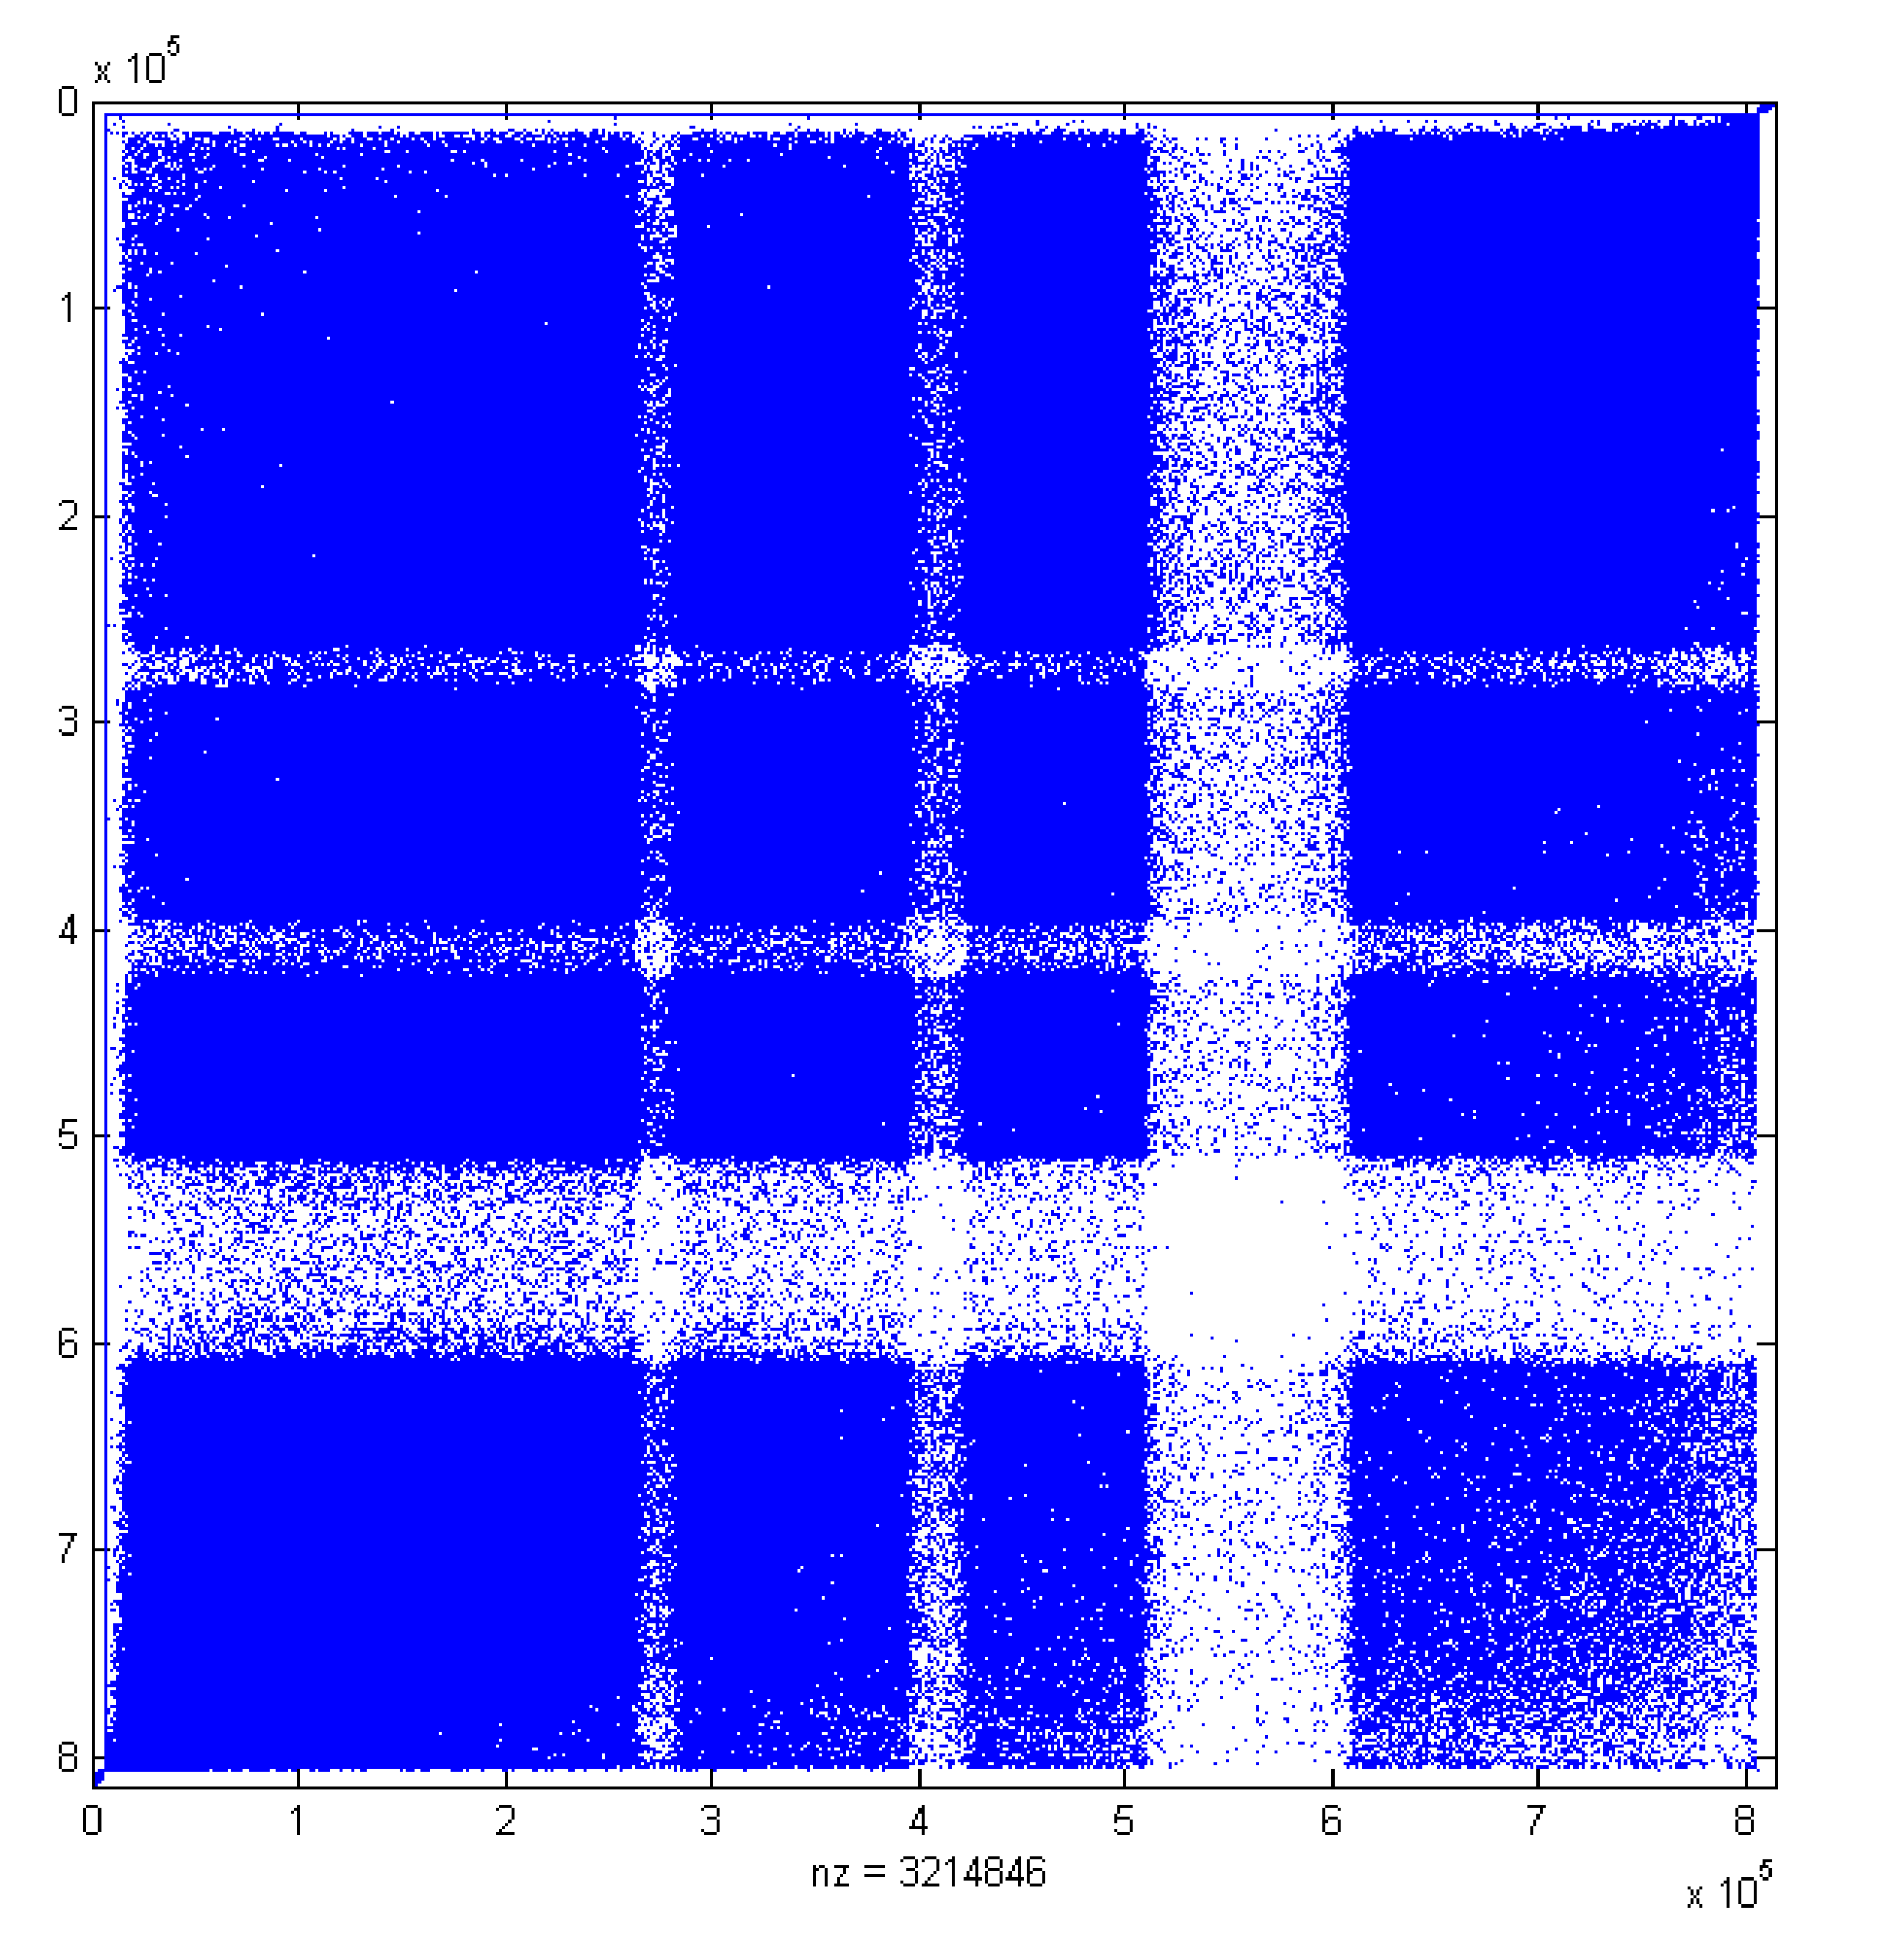
\includegraphics[width=0.45\textwidth]{Moria_2_clustered.pdf}
% where an .eps filename suffix will be assumed under latex,
% and a .pdf suffix will be assumed for pdflatex; or what has been declared
% via \DeclareGraphicsExtensions.
\caption{Rearranged Adjacency Matrix of Call Graph of Moria City in Month 2}
\label{Moria_2_clustered}
\end{figure}

From Figure \ref{Moria_2_clustered} we can observe that though some edges have been removed in the call graph of Moria city in month 2, the community structures in the call graph of Moria city haven't been changed much. In  Figure \ref{Moria_2_clustered}, we still can find the community structures which are similar to those in Figure \ref{Moria_1_clustered}. For instance, the vertices at the lower right corner in Figure \ref{Moria_2_clustered} and the vertices at the upper left corner in Figure \ref{Moria_1_clustered} are in the same community.   
